%Left to do.... 
% label fig 2

\documentclass{article}
\hyphenation{Post-Script} % tell LaTeX how to hyphenate certain words

%%%%%%%%%%%%
% PACKAGES %
%%%%%%%%%%%%
\usepackage[a4paper]{geometry}  % Please use A4 for all submissions
\usepackage{wimp}               % style
\usepackage{cite}               % smart citations (group, order...)
\usepackage{hyperref}           % clickable references and URLs
\usepackage{graphicx}           % figures
\graphicspath{{images/}}        % set default image folder
% insert any additional packages if necessary ...


%%%%%%%%%
% TITLE %
%%%%%%%%%
\title{Investigation into the origins of the phrase 'boop da snoot'}

%%%%%%%%%%%
% AUTHORS %
%%%%%%%%%%%
% comment out as needed

% SINGLE AUTHOR --------------------------
%\affiliation{Author 1}
%{Acoustics Research Centre \\
%University of Salford\\
%Salford, UK.\\
%{\tt author@salford.ac.uk}}
%----------------------------------------------------

% SEVERAL AUTHORS AT SAME INSTITUTION ----
\affiliation{Author 1, Author 2, Author 3}
{Interdisciplinary Centre for Computer Music Research\\ University of Plymouth\\
{\tt \{a1,a2,a3\}@plymouth.ac.uk}}
%----------------------------------------------------

% TWO AFFILIATIONS ----------------------------------
% \twoaffiliations{Author 1 and Author 2} % authors at first institution
% 	{Interdisciplinary Centre for Computer Music Research\\ University of Plymouth\\ {\tt \{a1,a2\}@qmul.ac.uk}} 
% 	{Author 3} % authors at second institution
% 	{Digital Media Technology Lab \\ Birmingham City University \\ {\tt a3@bcu.ac.uk}}
%----------------------------------------------------

% THREE AFFLILIATIONS -------------------------------
%\threeaffiliations
%{Author 1} % authors at second institution
%{Digital Media Technology Lab \\ Birmingham City University \\ Birmingham, UK \\ {\tt a1@bcu.ac.uk}}
%{Author 2} % authors at first institution
%{Centre for Digital Music \\ Queen Mary University of London \\ London, UK \\ {\tt a2@qmul.ac.uk}} 
%{Author 3} % authors at second institution
%{Interdisciplinary Centre for Computer Music Research\\ University of Plymouth\\{\tt a3@salford.ac.uk}}
%----------------------------------------------------

% FOUR AFFLILIATIONS --------------------------------
% \fouraffiliations
%{Author 1} % authors at second institution
%{Digital Media Technology Lab \\ Birmingham City University \\ Birmingham, UK \\ {\tt a1@bcu.ac.uk}}
%{Author 2} % authors at first institution
%{Centre for Digital Music \\ Queen Mary University of London \\ London, UK \\ {\tt a2@qmul.ac.uk}} 
%{Author 3} % authors at second institution
%{Interdisciplinary Centre for Computer Music Research\\ University of Plymouth\\{\tt a3@plymouth.ac.uk}}
%{Author 4} % authors at second institution
%{Interdisciplinary Centre for Computer Music Research\\ University of Plymouth\\{\tt a4@plymouth.ac.uk}}
%----------------------------------------------------

\begin{document}
\maketitle

%%%%%%%%%%%%
% ABSTRACT %
%%%%%%%%%%%%

\begin{abstract}
This is the template file for the proceedings of the 6\textsuperscript{th} Workshop on Intelligent Music Production (WIMP2020).
This template has been derived from WASPAA'99 templates and aims at producing workshop proceedings in electronic form.
The format is essentially the one used for ICASSP conferences.
Please use either this \LaTeX{} or the accompanying Word formats when preparing your submission.
The templates are available in electronic form on the workshop website.\footnote{\url{http://intelligent-music-production.github.io/}}
\end{abstract}

\section{Introduction}
\label{sec:intro}
This template can be found on the workshop website.

\subsection{Figures}
\label{ssec:figures}
All figures should be centred on the column (or page, if the figure spans both columns).
Figure captions (in italic) should follow each figure and have the format given in Figure \ref{fft_plot}.
%
Vectorial figures are preferred. For example when using
\texttt{Matlab}, export using either Postscript or PDF format. Also,
in order to provide a better readability, figure text font size
should be at least identical to footnote font size. To do so using
\texttt{Matlab}, use the \texttt{subplot} command before plotting.
If bitmap figures are used, please make sure that the resolution is
enough for print quality. Fig. \ref{ftt_plot2} illustrates an
example of a figure spanning two columns.
%
\begin{figure}[ht]
\centerline{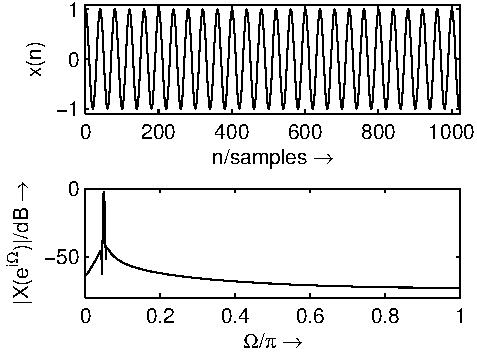
\includegraphics[scale=0.8]{fft_plot2}}
\caption{\label{fft_plot}{\it Sinusoid in time and frequency domain. Short captions are centered, long captions (more than 1 line) are justified.}}
\end{figure}
%
\begin{figure*}[ht]
\center
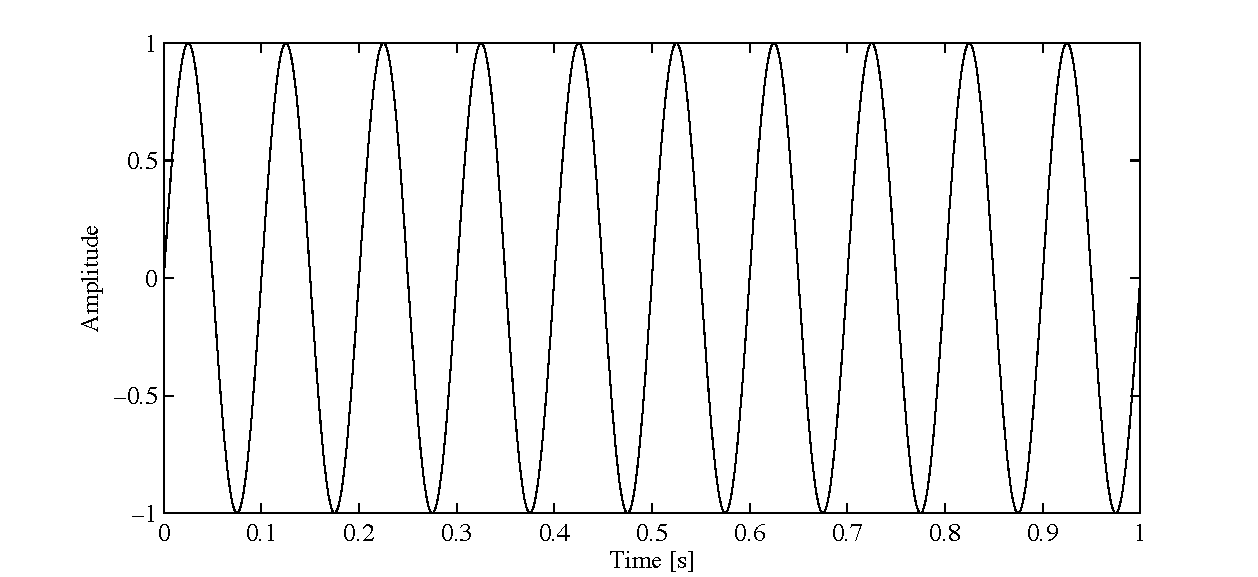
\includegraphics[width=5in]{TwoColumnSine2}
\caption{\label{ftt_plot2}{\it A figure spanning two columns, as mentioned in Sec. \ref{ssec:figures}. }}
\end{figure*}


\subsection{Tables}
As for figures, all tables should be centered on the column (or page, if the table spans both columns).
Table captions should be in italic, precede each table and have the format given in Table \ref{tab:example}.

\begin{table}[ht]
  \caption{\itshape Basic trigonometric values.}
	\centering
	\begin{tabular}{|c|c|}
		\hline
		$\mathrm{angle}\,(\theta, \mathrm{rad})$ & $\sin \theta$ \\\hline
		$\frac{\pi}{2}$ & $1$ \\
		$\pi$ & $0$ \\
		$\frac{3\pi}{2}$ & $-1$ \\
		$2\pi$ & $0$ \\\hline
	\end{tabular}
	%
	\label{tab:example}
\end{table}

\begin{table*}[ht]
  \caption{{\it Basic trigonometric values, spanning two columns.}}
	\centering
  \begin{tabular}{|c|c|c|c|c|c|c|}\hline
    $\mathrm{angle}\, (\theta, \mathrm{rad})$ & $\sin \theta$ & $\cos \theta $ & $(\sin \theta)/2 $ & $(\cos \theta) /2 $ & $(\sin \theta)/3 $ & $(\cos \theta)/3$    \\\hline
    $\frac{\pi}{2}$ & $1$ & $0$ & $1/2$ & $0$ & $1/3$ & $0$ \\
    $\pi$ & $0$ & $-1$ & $0$ & $-1/2$ & $0$ & $-1/3$\\
    $\frac{3\pi}{2}$ & $-1$ & $0$ & $-1/2$ & $0$ & $-1/3$ & $0$ \\
    $2\pi$ & $0$ & $1$ & $0$ & $1/2$ & $0$ & $1/3$ \\\hline
 \end{tabular}
	%
  \label{tab:example2}
\end{table*}

\subsection{Equations}
Equations should be placed on separate lines and numbered:

\begin{equation}
	X(e^{j\Omega})=\sum_{n=0}^{N-1}x(n)e^{-j\Omega n}
	\label{eq1}
	\end{equation}
	where the sequence $x(n)$ in equation (\ref{eq1}) is a windowed frame:
	\begin{equation}
	x(n)=s(n) w(n)
	\label{eq2}
\end{equation}
%
with a window function $w(n)$.


\subsection{Page Numbers}
Page numbers will be added to the document in the post-processing stage, so no number are expected to show on this document


\subsection{References}
The references will be numbered in order of appearance \cite{Mitra:Kaiser:1993:DSP:handbook}, \cite{Haykin:1991:adaptive:filter}, \cite{Moorer:2000:AES:audio:millenium} and \cite{Nackaerts:2001:ICMC}. Please avoid listing references that do not appear in the text (we did the opposite in this template).


\subsubsection{Reference Format}
The reference format is the standard IEEE one. We recommend to use BibTeX to create the reference list.


\section{Conclusions}
This template can be found on the workshop website.\footnote{\url{http://intelligent-music-production.github.io/}}
For changing the number of author affiliations (1 to 4), uncomment the corresponding regions in the template \texttt{tex} file.
Please, submit full-length papers (max.~4 pages both oral and poster presentations).
Submission system is to send papers directly by e-mail.

\section{Acknowledgments}
Many thanks to the great number of anonymous reviewers!

%%%%%%%%%%%%%%%%%%%%%%
%     REFERENCES     %
%%%%%%%%%%%%%%%%%%%%%%

\bibliographystyle{ieeetr}
\bibliography{bibliography}{}
% uncomment the lines below (and comment the line above) if you want to enter the bibliography manually
% \begin{thebibliography}{10}
% \bibitem{dugan1975automatic}
% D.~Dugan, ``Automatic microphone mixing,'' {\em Journal of the Audio
%   Engineering Society}, vol.~23, July/August 1975.
% \bibitem{case2011mixsmart}
% A.~Case, {\em Mix Smart: Professional Techniques for the Home Studio}.
% \newblock Focal Press, 2011.
% \bibitem{massenburg1972parametric}
% G.~Massenburg, ``Parametric equalization,'' in {\em 42nd Convention of the
%   Audio Engineering Society}, May 1972.
% \bibitem{mushra}
% {\em Method for the subjective assessment of intermediate quality level of
%   coding systems}.
% \newblock Recommendation {ITU-R BS.1534-1}, 2003.
% \end{thebibliography}
\end{document}
